\chapter{代数}

\section{不等式}

已知 $a,b,c,d$ 为正实数, 求证
\[22a + 25b + 30c + 30d \ge 360 \sqrt[3]{\frac{abcd}{2a+5b+10c+30d}},\]
并确定等式成立的条件.

证明: 

\begin{align*}
2a+5b+10c+30d &=10\cdot\frac{a}{5}+20\cdot\frac{b}{4}+30\cdot\frac{c}{3}+60\cdot\frac{d}{2} \\
& \ge 120\sqrt[120]{\left(\frac{a}{5}\right)^{10}\cdot\left(\frac{b}{4}\right)^{20}\cdot\left(\frac{c}{3}\right)^{30}\cdot\left(\frac{d}{2}\right)^{60}}\\
&= 120\sqrt[12]{\left(\frac{a}{5}\right)\cdot\left(\frac{b}{4}\right)^2\cdot\left(\frac{c}{3}\right)^3\cdot\left(\frac{d}{2}\right)^6}
\end{align*}

所以
\begin{align*}
\sqrt[3]{\frac{abcd}{2a+5b+10c+30d}} &\le \sqrt[3]{\frac{abcd}{120\sqrt[12]{(\frac{a}{5})\cdot(\frac{b}{4})^2\cdot(\frac{c}{3})^3\cdot(\frac{d}{2})^6}}} \\
&= \sqrt[36]{\frac{a^{11}\cdot b^{10}\cdot c^9\cdot d^6}{2^{26}\cdot 3^9\cdot 5^{11}}} \\
&= \sqrt[36]{\left(\frac{a}{5}\right)^{11}\cdot\left(\frac{b}{4}\right)^{10}\cdot\left(\frac{c}{3}\right)^{9}\cdot\left(\frac{d}{2}\right)^6}\\
\end{align*}

进而
\begin{align*}
22a+25b+30c+30d &= 10\cdot\left[11\cdot(\frac{a}{5})+10\cdot(\frac{b}{4})+9\cdot(\frac{c}{3})+6\cdot(\frac{d}{2})\right] \\
&\ge 10\cdot 36\sqrt[36]{\left(\frac{a}{5}\right)^{11}\cdot\left(\frac{b}{4}\right)^{10}\cdot\left(\frac{c}{3}\right)^{9}\cdot\left(\frac{d}{2}\right)^6}\\
&\ge 360 \sqrt[3]{\frac{abcd}{2a+5b+10c+30d}}
\end{align*}

等号在 $a:b:c:d=5:4:3:2$ 时取得.

~
\newpage
%------------------------------------------------------------------------------%

\noindent A.Oppenheim 不等式

设 $a,b,c,S$ 分别为 $\triangle ABC$ 的三边长和面积, 则对任意 $x,y,z\in R$ 有
\[(xa^2+yb^2+zc^2)^2 \ge 16S^2(xy+yz+zx) .\]
等号成立当且仅当 $a^2:b^2:c^2=(y+z):(z+x):(x+y)$.

\begin{wrapfigure}[4]{o}{0pt}
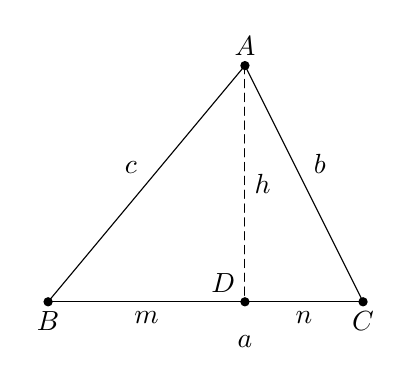
\begin{tikzpicture}[cap=round,scale=1]
\tikzstyle{axes}=[line width=1pt]
\coordinate[label=135:$D$,] (D) at (0.0,0.0);
\coordinate[label=below:$B$] (B) at (-2.5,0.0);
\coordinate[label=below:$C$] (C) at (1.5,0.0);
\coordinate[label=above:$A$] (A) at (0.0,3.0);
\draw[] (B) to [edge label = $c$] (A);
\draw[] (A) to [edge label = $b$] (C);
\draw[] (C) to [edge label = $n$] (D);
\draw[] (D) to [edge label = $m$] (B);
\draw[densely dashed] (A) to [edge label = $h$] (D);
\foreach \p in {A,B,C,D}
	\fill[fill=black,draw=black,thick] (\p) circle (1.25pt);
\draw[] (0,-0.5) node {$a$};
\tkzMarkRightAngle[line width=1pt](A,D,C);
\end{tikzpicture}
\end{wrapfigure}
~

\begin{proof}
如图, 过$A$点作$BC$边上的高 $AD=h$, 有
\begin{align*}
 k&=xa^2+yb^2+zc^2\\
&=x(m+n)^2+y(n^2+h^2)+z(m^2+h^2)\\
&=x(m+n)^2+(yn^2+zm^2)+(y+z)h^2\\
&\ge x(m+n)^2+\frac{(m+n)^2}{\frac{1}{y}+\frac{1}{z}}+(y+z)h^2\\
&= \frac{xy+yz+zx}{y+z}(m+n)^2+(y+z)h^2\\
&\ge 2\sqrt{xy+yz+zx}(m+n)h\\
&=4\sqrt{xy+yz+zx}\cdot S
\end{align*}

两个不等号分别使用了权方和不等式(或柯西不等式变形)及均值不等式.

于是, $S\le \dfrac{k}{4\sqrt{xy+yz+zx}}$, 等号成立当且仅当 $a^2:b^2:c^2=(y+z):(z+x):(x+y)$.
\end{proof}

~

\noindent 补充:

事实上, 第一个不等号只要用到权方和不等式的特殊形式即可: 
\begin{align*}
\left(\frac{1}{y}+\frac{1}{z}\right)(ym^2+zn^2) &= m^2 + n^2 + \frac{y}{z}m^2 + \frac{z}{y}n^2\\
&\ge m^2+n^2 + 2\sqrt{\frac{y}{z}m^2\cdot\frac{z}{y}n^2}\\
&=(m+n)^2
\end{align*}
于是有 
\[
(ym^2+zn^2) \ge \frac{(m+n)^2}{\frac{1}{y}+\frac{1}{z}}.
\]

\newpage
%------------------------------------------------------------------------------%
若 $\triangle ABC$ 的三边 $a,b,c$ 满足 $a^2+b^2+3c^2=7$, 求 $\triangle ABC$ 面积的最大值.

~

\noindent 解法一: 可以直接用 A.Oppenheim 不等式, 令$x=1,y=1,z=3$, 则
\[S\le\frac{xa^2+yb^2+zc^2}{4\sqrt{xy+yz+zx}} = \frac{\sqrt{7}}{4}. \]

~

\noindent 解法二: 由三角形面积公式, 以余弦定理:
\begin{align*}
S &= \frac{1}{2}ab\sin C \\
&= \frac{1}{2}ab\sqrt{1-\cos^2 C}\\
&= \frac{1}{2}ab\sqrt{1-\left(\frac{a^2+b^2-c^2}{2ab}\right)^2}\\
&= \frac{1}{2}\sqrt{(ab)^2-\frac{(a^2+b^2-c^2)^2}{4}}\\
&=\frac{1}{2}\sqrt{(ab)^2-\frac{(7-4c^2)^2}{4}}
\end{align*}
又因为 $ab\le\dfrac{a^2+b^2}{2}=\dfrac{7-3c^2}{2}$, 所以
\begin{align*}
S &=\frac{1}{2}\sqrt{(ab)^2-\frac{(7-4c^2)^2}{4}}\\
& \le\frac{1}{2}\sqrt{\frac{(7-3c^2)^2}{4}-\frac{(7-4c^2)^2}{4}}\\
&= \frac{1}{4}\sqrt{-7(c^2-1)^2+7}\\
&\le \frac{\sqrt{7}}{4}.
\end{align*}

~

\noindent 解法三: 设 $D$ 是 $AB$ 的中点, 由三角形中线长公式: $\displaystyle CD = \frac{1}{2}\sqrt{2(a^2+b^2)-c^2}$.

即 $4CD^2 + c^2 = 2(a^2+b^2)$, 而 $a^2+b^2+3c^2=7$, 所以
\[2CD^2+\frac{7}{2}c^2=a^2+b^2+3c^2=7.\]
等式左边根据均值不等式有: 
\[2CD^2+\frac{7}{2}c^2 \ge 2\sqrt{7}CD\cdot c\ge 2\sqrt{7}h_c\cdot c.\]
所以 $S=\dfrac{1}{2}h_c\cdot c \le \dfrac{1}{2}\cdot\dfrac{7}{2\sqrt{7}}=\dfrac{\sqrt{7}}{4}.$

\newpage
%------------------------------------------------------------------------------%
\section{函数}

\noindent 2019南京大学计算机拔尖班二次选拔:

假设$f$是定义在正整数集合上, 取值也总是正整数的一个函数, 并且满足对于任意的正整数 $m,n$, 若 $m-n$ 也是正整数, 那么 $f(m+n)f(m-n)=f(m^2)$, 求所有满足条件的函数 $f$.

~

解: 先取$n=1,2$, 有:
\[ f(m+1)f(m-1) = f(m^2) = f(m+2)f(m-2) .\]
于是得到: $\dfrac{f(m+2)}{f(m+1)} = \dfrac{f(m-1)}{f(m-2)}$. 

可以看出$\dfrac{f(m+2)}{f(m+1)}$ 的值是周期为 3 的序列. 按 $x$ 模3 的余数, 分别讨论$f(x)$:

(a) 若 $x=3k$, 则 $\dfrac{f(3k+2)}{f(3k+1)} = \dfrac{f(3k-1)}{f(3k-2)} = \cdots = \dfrac{f(5)}{f(4)} = \dfrac{f(2)}{f(1)}$, 所以
\[f(3k+2) = \dfrac{f(2)}{f(1)}f(3k+1) .\]

(b) 若 $x=3k+1$, 则 $\dfrac{f(3k+3)}{f(3k+2)} = \dfrac{f(3k)}{f(3k-1)} = \cdots = \dfrac{f(6)}{f(5)} = \dfrac{f(3)}{f(2)}$, 所以
\[f(3k+3) = \dfrac{f(3)}{f(2)}f(3k+2) .\]

(c) 若 $x=3k-1$, 则 $\dfrac{f(3k+1)}{f(3k)} = \dfrac{f(3k-2)}{f(3k-3)} = \cdots = \dfrac{f(7)}{f(6)} = \dfrac{f(4)}{f(3)}$, 注意到取 $m=2$, $n=1$时, 根据题目条件有$f(3)f(1)=f(4)$, 所以
\[f(3k+1) = \dfrac{f(4)}{f(3)}f(3k) = f(1)f(3k) .\]

综合 (a)(c) 有: $f(3k+2)=f(2)f(3k)$; 

综合 (a)(b)(c) 有: $f(3k+3) = f(3)f(3k)$. 这意味着 $f(3k)$ 是一个等比数列, 通项公式为 $f(3k)=f(3)^k$.

进一步有: $f(3k+2)=f(2)f(3)^k, f(3k+1) = f(1)f(3)^k$

回到原条件, 取 $m=3k$, $n=1$, 得 
\begin{align*}
f(3k+1)f(3k-1) &=f(9k^2) \\
f(1)f(3)^k \cdot f(2)f(3)^{k-1} &= f(3)^{3k^2}\\
f(1)f(2) &= f(3)^{3k^2-2k+1}
\end{align*} 
$f(1)f(2)$ 是定值, 说明 $f(3)^{3k^2-2k+1}$ 对任意的 $k$ 都是定值, 于是只有 $f(3)=1$. 

而 $f(1), f(2)$ 都是整数, 并且$f(1)f(2)=1$, 因此必有 $f(1)=f(2)=1$.

所以满足题目条件的函数只有 $f(x)=1$.


\newpage
%------------------------------------------------------------------------------%
\noindent 2022中科大少年班复试

记 $g(x)=x^2-k$, $h(x)=g(g(x))$, $k$ 为整数.

(1) 写出$h(x)$ 的表达式;

(2) 求集合 $A=\{ x\in \mathbb{R} | h(x) = x\}$;

(3) 已知函数 $f: A\rightarrow A$ 满足 $f(f(x)) = g(x)$, 证明: $f$ 既是单射也是满射;

(4) 是否存在函数 $s(x)$, 使得$s(s(x))=x^2-2$, 证明你的结论.

~

\noindent 解: 

(1)\ \ \ $h(x) = (x^2-k)^2-k$.

~

(2)\ \ \ 当 $g(x)=x$ 时, $h(x)=g(g(x))=x$, 意味着 $g(x)-x=0$ 的根也属于集合 $A$. 于是可以进行因式分解:
\[ h(x)-x =  (x^2-k)^2-k - x = (x^2-x-k)(x^2+x+1-k) \]
两项的判别式分别是 $\Delta_1 = 1+4k$, $\Delta_2 = 1-4(1-k)=4k-3$. 令
\[x_{1,2}=\frac{1\pm\sqrt{\Delta_1}}{2},\qquad x_{3,4}=\frac{-1\pm\sqrt{\Delta_2}}{2} ,\]
考虑到$k$是整数,
当 $k < -\dfrac{1}{4}$ 时, $A=\varnothing$;
当 $-\dfrac{1}{4} < k < \dfrac{3}{4}$ 时, $A=\{x_1, x_2\}$;
当 $k > \dfrac{3}{4}$ 时, $A=\{x_1, x_2, x_3, x_4\}$.

~

(3)\ \ \ 先证单射: 若 $a,b\in A$, 且满足 $f(a)=f(b)$, 则 $g(a)=f(f(a))=f(f(b))=g(b)$, 进一步有 $h(a)=g(g(a))=g(g(b))=h(b)$, 由 $a,b\in A$ 得 $h(a)=a$ 和 $h(b)=b$, 所以推出 $a=b$, 于是单射得证.

~

再证满射: 对任意 $a\in A$, 有 $a = h(a)=g(g(a))=f(f(f(f(a))))$, 只要取 $x = f(f(f(a)))$, 可知$x\in A$, 并且有 $f(x)=a$. 于是满射也得证.

(4)\ \ \ $g(x)=x^2-2$, $A$ 中存在 4 个元素, 分别为 $x_1 = -1$, $x_2=2$, $x_3=\dfrac{-1-\sqrt{5}}{2}$, $x_4=\dfrac{-1+\sqrt{5}}{2}$. 可以直接计算验证 $g(x_1)=x_1$, $g(x_2)=x_2$, $g(x_3)=x_4$, $g(x_4)=x_3$. 

根据第(3)问, 若存在 $s(x)$, 使得 $s(s(x))=g(x)$, 则 $s: A\rightarrow A$ 是一个双射函数. 看看$s$ 将 $x_3$ 映射到多少. 

假设$s(x_3)=x_3$, 则 $g(x_3)=s(s(x_3))=x_3$, 这与 $g(x_3)=x_4$ 矛盾.

假设$s(x_3)=x_4$, 那么因为 $s$ 是双射, 所以$s(x_4)\ne x_4$, 于是 $g(x_3)=s(s(x_3))=s(x_4)\ne x_4$, 同样与 $g(x_3)=x_4$ 矛盾.

假设$s(x_3)=x_1$, 则 $x_4 = g(x_3)=s(s(x_3))=s(x_1)$, 两边再用 $s$ 作用得: $s(x_4) = s(s(x_1)) = g(x_1)=x_1=s(x_3)$, 与$s$ 是双射矛盾. 

假设$s(x_3)=x_2$, 跟上一条类似.

所以不存在这样的 $s$.


\newpage
%------------------------------------------------------------------------------%
\noindent 半群一定存在幂等元:

设 $A$ 是有限集, 定义运算$\otimes$满足:

(1) 封闭性: 对任意 $x,y\in A$, 有 $x\otimes y\in A$;

(2) 结合律: 对任意 $x,y,z\in A$, 有 $(x\otimes y)\otimes z = x\otimes(y\otimes z)$.

证明: 存在$\alpha\in A$, 使得 $\alpha\otimes\alpha=\alpha$.


~

解: 固定 $x\in A$, 若 $x\otimes x = x$, 则已经找到幂等元, 否则, 可以构造序列 $\{a_n\}$, 其中 $a_1=x\otimes x$, $a_{n}=a_{n-1}\otimes a_{n-1}$. 因为 $\otimes$ 满足封闭性, 所以序列 $\{a_n\}$ 是 $A$ 的子集, 而 $A$  是有限集, 所以 $\{a_n\}$ 必然有重复元素, 于是可以设 $a_s = a_t, s<t$. 再取出之间的一段作为序列$\{b_m\}$, 即
\begin{align*}
b_1&=a_s,\\ 
b_2&=a_{s+1}=b_1\otimes b_1 = b_1^2,\\ 
b_3&=a_{s+2}=b_2\otimes b_2 = b_1^4,\\
&\cdots\\ 
b_m&=a_{t-1} = b_{m-1}\otimes b_{m-1} = b_1^{2^{m-1}},\\
b_1&=a_t=b_{m}\otimes b_m=b_1^{2^m}.
\end{align*}
上述等式从第二行往下, 左边有一个 $b_1, \cdots, b_m$, 右边有两个, 考虑将它们乘起来.
\[b_2\otimes b_3\otimes\cdots b_m\otimes b_1 = (b_1\otimes b_1)\otimes(b_2\otimes b_2)\otimes\cdots(b_m\otimes b_m).\]
用$b_1$ 表示 $b_2,\cdots,b_m$, 再根据结合律, 可以发现其实 $\{b_1, \cdots, b_m\}$ 之间的运算是满足交换律的. 上式左边等于 $b_1^{2+4+\cdots+2^{m-1}+1}$, 右边等于 $b_1^{2+4+\cdots+2^m}$, 于是只要令 $y=b_2\otimes b_3\otimes\cdots b_m\otimes b_1$, 就有 $y=y\otimes y$, 也就构造出了幂等元.

~

解法2: 固定 $x\in A$, 由于 $A$ 是有限集且具有封闭性, 所以存在 $s,t\in\mathbb{N}$, 使得 $x^s = x^{s+t}$, 从而对任意正整数 $k$, 当 $k\ge s$ 时, 都有 $x^k=x^{k+t}$. 这样, 当 $k\ge s$ 时, $x^k=x^{k+t}=x^{k+2t}=\cdots=x^{k+mt}$ 对任意 $m$ 都成立.

取$k$是$t$ 的倍数$k=qt$, $q\in\mathbb{N}^+$, 并且$q$足够大, 满足 $k\ge s$, 于是
\[ (x^k)^2 = x^{qt}\otimes x^k=x^{qt+k}=x^k .\]
这样, $\alpha=x^k$ 满足 $\alpha^2=\alpha$.

\newpage
%------------------------------------------------------------------------------%
\noindent $\sqrt{2}$ 是无理数的一种奇特证法

因为 $1<\sqrt{2}<2$, 有 $0<\sqrt{2}-1<2$. 考虑序列 $s_n = (\sqrt{2}-1)^n$, 它总是具有 $A_n\sqrt{2}+B_n$ 的形式. 这里 $A_n, B_n$ 都是整数.

倘若 $\sqrt{2}$ 是有理数, 设 $\sqrt{2} = p/q$, 其中 $p,q$ 是正整数. 则 $A_n\sqrt{2}+B_n$ 的分母是 $q$, 且 $s_n>0$, 从而 $s_n \ge 1/q$. 但是 $s_n$ 是趋于 0 的, 矛盾.

\newpage
%------------------------------------------------------------------------------%

\noindent 来自网络

求和
\[ 
S = \sum_{a_1=0}^{\infty}\sum_{a_2=0}^{\infty}\cdots\sum_{a_7=0}^{\infty}{\frac{a_1+a_2+\cdots+a_7}{3^{a_1+a_2+\cdots+a_7}}}
\]

解: 将求和号合并, 再由对称性, 可得
\begin{align*}
S &= \sum_{a_1,\cdots,a_7} {\frac{a_1}{3^{a_1+a_2+\cdots+a_7}} + \frac{a_2}{3^{a_1+a_2+\cdots+a_7}} + \cdots + \frac{a_7}{3^{a_1+a_2+\cdots+a_7}}} \\
 &= 7\cdot\sum_{a_1,\cdots,a_7} {\frac{a_1}{3^{a_1+a_2+\cdots+a_7}}}
\end{align*}
再将求和号拆开, 得到:
\begin{align*}
S &= 7\cdot \sum_{a_1=0}^{\infty}\sum_{a_2=0}^{\infty}\cdots\sum_{a_7=0}^{\infty}{\frac{a_1}{3^{a_1+a_2+\cdots+a_7}}} \\
&=  7\cdot \sum_{a_1=0}^{\infty}\frac{a_1}{3^{a_1}}\cdot\left(\sum_{a_2=0}^{\infty}\cdots\sum_{a_7=0}^{\infty}{\frac{1}{3^{a_2}}\cdots\frac{1}{3^{a_7}}}\right)\\
&= 7\cdot \sum_{a_1=0}^{\infty}\frac{a_1}{3^{a_1}}\cdot\left(\sum_{a_2=0}^{\infty}{\frac{1}{3^{a_2}}}\right)^6
\end{align*}
两部分分别求和, 其中易求得
\[
S_1 = \sum_{a_1=0}^{\infty}\frac{a_1}{3^{a_1}} = \frac{3}{4}
\]
以及 
\[ S_2 = \sum_{a_2=0}^{\infty}\frac{1}{3^{a_2}} = \frac{3}{2}
\]
所以 
\[
S = 7\cdot\frac{3}{4}(\frac{3}{2})^6 = \frac{7\cdot 3^7}{2^8}
\]


\newpage
%------------------------------------------------------------------------------%

\noindent 堆垒求和方法
\[ S(n,k) = \sum_{i=1}^{n}{i^k} \]

首先, $ k = 1 $ 时, \[ S(n,1) = 1 + 2 + \cdots + n = \frac{(n+1)n}{2} .\]

当 $ k = 2 $ 时, 因为
\begin{align*}
(n+1)^3 &= n^3 + 3n^2 + 3n + 1 \\ 
n^3 &= (n-1)^3 + 3(n-1)^2 + 3(n-1) + 1\\
\cdots & \\
 2^3 &= 1^3 + 3\cdot 1^2 + 3\cdot 1 + 1
\end{align*}

两边全部加起来, 得到: 
\begin{align*} 
(n+1)^3 &= 1 + 3\cdot(1^2+2^2+\cdots+n^2) + 3\cdot(1+2+\cdots+n) + n \\
	&= 1 + 3S(n,2) + 3S(n,1) + n\\
3S(n,2) &= (n+1)^3 - 3S(n,1) - n - 1 \\
	S(n,2) &= \frac{n(n+1)(2n+1)}{6} .
\end{align*}

当 $ k = 3 $ 时, 有:
\begin{align*} 
(n+1)^4 &= n^4 + 4n^3 + 6n^2 + 4n + 1 \\
		&= 1 + 4S(n,3) + 6S(n,2) + 4S(n,1) + n
\end{align*} 

也可以同理推出来.

\newpage
%------------------------------------------------------------------------------%
求和: 
$\displaystyle \sum_{n=1}^{\infty}{\frac{n^3}{2^n}}$ .

\noindent 反复利用堆垒求和即可. 令 $S_k$ = $\displaystyle \sum_{n=1}^{\infty}{\frac{n^k}{2^n}}$, 则:
\begin{align*}
S_0 &= \sum_{n=1}^{\infty}{\frac{1}{2^n}} = 1 \\
S_1 &= \sum_{n=1}^{\infty}{\frac{n}{2^n}} \\
2S_1 &= \sum_{n=1}^{\infty}{\frac{n}{2^{n-1}}} = 1+\sum_{n=1}^{\infty}{\frac{n+1}{2^{n}}} \\
&= 1+\sum_{n=1}^{\infty}{\frac{n}{2^{n}}} + \sum_{n=1}^{\infty}{\frac{1}{2^{n}}} = 1 + S_1 + S_0\\
S_1 &= 2 \\
S_2 &= \sum_{n=1}^{\infty}{\frac{n^2}{2^n}} \\
2S_2 &= \sum_{n=1}^{\infty}{\frac{n^2}{2^{n-1}}} = 1 + \sum_{n=1}^{\infty}{\frac{(n+1)^2}{2^n}}\\ 
&= 1 + \sum_{n=1}^{\infty}{\frac{n^2}{2^n}} + \sum_{n=1}^{\infty}{\frac{2n}{2^n}} + \sum_{n=1}^{\infty}{\frac{1}{2^n}} = 1 + S_2 + 2S_1 + S_0 \\
S_2 &= 6 \\
S_3 &= \sum_{n=1}^{\infty}{\frac{n^3}{2^n}} \\
2S_3 &=   \sum_{n=1}^{\infty}{\frac{n^3}{2^{n-1}}} = 1 + \sum_{n=1}^{\infty}{\frac{(n+1)^3}{2^n}} \\
&= 1 +  \sum_{n=1}^{\infty}{\frac{n^3}{2^n}} +  \sum_{n=1}^{\infty}{\frac{3n^2}{2^n}} +  \sum_{n=1}^{\infty}{\frac{3n}{2^n}} +  \sum_{n=1}^{\infty}{\frac{1}{2^n}} \\
&= 1 + S_3 + 3S_2 + 3S_1 + S_0\\
S_3 &= 26
\end{align*}

~

\noindent 也可以用生成函数的方法. 令 
\[f(x) =  \sum_{n=1}^{\infty}{\frac{x^n}{2^n}} = \frac{x}{2-x} ,\]
则对 $f(x)$ 求导, 并继续构造, 依次可以得到:
\begin{align*}
f'(x) &=  \sum_{n=1}^{\infty}{\frac{n\cdot x^{n-1}}{2^n}} = \left( \frac{x}{2-x} \right)' = \frac{2}{(2-x)^2} \\
g(x) &= x\cdot f'(x) = \sum_{n=1}^{\infty}{\frac{n\cdot x^n}{2^n}} = \frac{2x}{(2-x)^2} \\
g'(x) &= \sum_{n=1}^{\infty}{\frac{n^2 \cdot x^{n-1}}{2^n}} = \frac{4+2x}{(2-x)^3} \\
h(x) &= x\cdot g'(x) = \sum_{n=1}^{\infty}{\frac{n^2\cdot x^n}{2^n}} = \frac{4x+2x^2}{(2-x)^3} \\
h'(x) &= \sum_{n=1}^{\infty}{\frac{n^3\cdot x^{n-1}}{2^n}} = \frac{(4+4x)(2-x)+3(4x+2x^2)}{(2-x)^4}
\end{align*}

令 $x=1$, 代入 $h'(x)$, 得到
\[h'(1) = \sum_{n=1}^{\infty}{\frac{n^3}{2^n}} = 26 .\]

\newpage
%------------------------------------------------------------------------------%

\noindent 生成函数, 多项式系数, 以及集合计数

\noindent 问题: 集合 $\{1,2,\cdots ,2000\}$ 的所有子集中, 元素之和能被 5 整除的子集有多少个. (来自 102 Combinatorial Problems From the Training of the USA IMO Team)

~

\noindent 解: 考虑多项式 
\begin{align*}
f(x) &= (1+x)(1+x^2)(1+x^3)\cdots(1+x^{2000}) \\
&= c_0 + c_1x + c_2x^2 + \cdots .
\end{align*}
它的展开式中 $x^n$ 的系数 $c_n$ 对应了和为 $n$ 的子集个数. 因为对于子集 $\{a_1, a_2, \cdots, a_m\}$ 和展开式中的项 $x^{a_1}x^{a_2}\cdots x^{a_m}$ 存在一一映射. 所以我们要寻找形如 $x^{5k}$ 项的系数之和.

可以取不同的 $x$, 并求和, 依次来消掉一些项, 例如, $f(1)+(f-1) = 2(c_0+c_2+c_4+\cdots)$, 就消去了奇数项, 从而可以求出偶数项系数之和.

类似地, 令 $ \xi = e^{2\pi i/5}$ 为 5 次单位根, 即 $\xi^5 = 1$, 易知 $1+\xi+\xi^2+\xi^3+\xi^4=0$. 而当$x = \xi, \xi^2, \xi^3, \xi^4$ 时, 集合 $\{x, x^2, x^3, x^4\} = \{\xi, \xi^2, \xi^3, \xi^4\}$. 所以
\begin{align*}
\sum_{n=0}^4{f(\xi^n)} &= 5c_0 + c_1(1+\xi+\xi^2+\xi^3+\xi^4)+c_2(1+\xi+\xi^2+\xi^3+\xi^4) + \cdots \\
&= 5(c_0+c_5+c_{10} + \cdots ).
\end{align*}
这样就只留下了 5 的倍数次幂的系数.

那么 $\displaystyle \sum_{n=0}^4{f(\xi^n)}$ 究竟是多少呢? 因为 $\xi^n$ 的幂次的值以 5 为周期, 即$\xi^{(m+5k)n}=\xi^{mn}$, 所以$f(\xi^n)$只是 5 个不同的数重复乘了 400 次, 即 
\[f(\xi^n)=\left[(1+\xi^n)(1+\xi^{2n})\cdots(1+\xi^{5n})\right]^{400}\]
当 $n=1,2,3,4$ 时,
\[f(\xi^n) = \left[(1+\xi)(1+\xi^{2})\cdots(1+1)\right]^{400}.\]
当 $n=0$ 时, $f(\xi^n)=2^{2000}$.

又因为 $\xi, \xi^2, \cdots, \xi^5$ 是 $g(x)=x^5-1$ 的 5 个根, 所以有如下的因式分解:
\[g(x) = x^5-1=(x-\xi)(x-\xi^2)(x-\xi^3)(x-\xi^4)(x-\xi^5).\]
将 $x=-1$ 代入 $g(x)$ 得 $-2 = -2(1+\xi)(1+\xi^2)(1+\xi^3)(1+\xi^4)$, 于是所有 5 次项的系数之和为
\[\frac{1}{5}\sum_{n=0}^4{f(\xi^n)}=\frac{1}{5}\left(4\times 2^{400}+2^{2000}\right) = \frac{1}{5}\left(2^{402}+2^{2000}\right).\]


\newpage
%------------------------------------------------------------------------------%
\noindent 生成函数例子:

~

\noindent 问题: 求斐波那契数列通项公式.

\noindent 解: 递推关系为: $F_0=0, F_1=1, F_n = F_{n-1} + F_{n-2}$, 生成函数为 
\[
G(x) = \sum_{n=0}^\infty{F_nx^n} .
\]

根据递归关系, 有 $ F_nx^n = F_{n-1}x^n+F_{n-2}x^n $, 对 $n$ 求和得:
\[
\sum_{n=2}^{\infty}{F_nx^n} = \sum_{n=1}^{\infty}{F_{n-1}x^n} + \sum_{n=2}^{\infty}{F_{n-2}x^n} ,
\]
将求和式换成 $G(x)$ 得:
\[
G(x) - x = xG(x) + x^2G(x) ,
\]
所以 $G(x) = \dfrac{x}{1-x-x^2}$. 设 $1-x-x^2=0$的两个根为 $r,s$, 那么
\[
G(x) = \frac{1}{r-s}\left(\frac{1}{1-rx} - \frac{1}{1-sx}\right) .
\]
而对于任意$\alpha$, 有 
\[\frac{1}{1-\alpha x} = 1+\alpha x+\alpha^2x^2 + \alpha^3x^3 + \cdots\]
所以
\[
G(x) = \frac{1}{r-s}((r-s)x + (r^2-s^2)x^2 + (r^3-s^3)x^3 + \cdots) \\
\]

对比 $x^n$ 的系数, 可以得到通项公式为 $F_n = \dfrac{r^n - s^n}{r-s}$, 由求根公式解得 $r=\dfrac{\sqrt{5}+1}{2}, s=\dfrac{\sqrt{5}-1}{2}$, 所以通项公式为:
\[F_n = \frac{1}{\sqrt{5}}\left( \left(\frac{\sqrt{5}+1}{2} \right)^n - \left(\frac{\sqrt{5}-1}{2} \right)^n \right)\]

~

~

问题: 求 $x_1 + x_2 + \cdots + x_k = n, (n\ge k)$ 的非负整数解个数.

解: 设 $f(x) = (1+x+x^2+x^3+\cdots)^k$, 则 $f(x)$ 的展开式的每一项的形式为 $x^{m_1}x^{m_2}\cdots x^{m_k}$, 所以一组满足 $m_1+m_2+\cdots+m_k=n$ 的组合对应一组解, 所有非负整数解的个数就是 $x^n$ 项的系数.

而另一方面, 对 $ f(x) = (1+x+x^2+x^3+\cdots)^k = \dfrac{1}{(1-x)^k}$ 做泰勒展开, 得到 $x^n$ 项系数为
\[
a_n = \frac{f^{(n)}(0)}{n!} = \frac{k\cdot(k+1)\cdots(k+n-1)}{n!} = C^{k-1}_{n+k-1}.
\]
这也就是原方程非负整数解的个数.

~

~

问题: 连续掷 10 次骰子, 求所得点数之和为 30 的概率.

解: 设 $a_n$ 为所得点数之和为 $n$ 的可能的情况数, 则数列 $\{a_n\}$ 的生成函数为
\[
f(x) = (x^1+x^2+x^3+x^4+x^5+x^6)^{10} = x^{10}\left(\frac{1-x^6}{1-x}\right)^{10}
\]
对 $(1-x^6)^{10}$ 做二项式展开, 并对 $(1-x)^{-10}$ 做泰勒展开, 可得
\[
f(x) = x^{10}\cdot\sum_{n=0}^{10}{(-1)^nC_{10}^nx^{6n}} \cdot \sum_{n=0}^{\infty}{C_{9+n}^9x^n},
\]
于是 $x^{30}$ 的系数为 $a_{30} = C_{10}^0\cdot C_{29}^9 - C_{10}^1\cdot C_{23}^9 + C_{10}^2\cdot C_{17}^9 - C_{10}^3\cdot C_{11}^2 = 2930455$ .


\newpage
%------------------------------------------------------------------------------%
求正整数 $ x $,$ y $ 和素数 $ p $,满足 $ x^3+y^3=p^2 $。

解:由 
\begin{equation*}
p^2=x^3+y^3=(x+y)(x^2-xy+y^2 )
\end{equation*}

知 $ p=x+y=x^2-xy+y^2 $,或写成 $ x^2-(y+1)x+(y^2-y)=0 $。

对 $ x $ 用求根公式,则
\[ 
x=\frac{(y+1)\pm\sqrt{(y+1)^2-4(y^2-y)}}{2} 
\]

根号内满足:$ (y+1)^2-4(y^2-y)=6y-3y^2+1\ge 0 $,所以 $ y $ 只可能取 1 或 2。

$ y=1 $ 时,$ x=2 $;$ y=2 $ 时,$ x=1 $;这两个解都满足。

\newpage
%------------------------------------------------------------------------------%
问题: $ [a] $ 表示不大于 $ a $ 的最大整数。自然数 $ n $ 满足:$ n=[n/2]+[n/3]+\cdots +[n/2010] $,求所有符合条件的 $ n $。

解:首先 $ n $ 一定小于 2010。所以 $ n=[n/2]+[n/3]+\cdots +[n/n] $。

可是又有 $ [n/2],[n/3],\cdots [n/n] $ 都至少为 1,而右边有 $ n-1 $ 项,所以有 $ [n/2]=2 $,其他项都等于 1,于是 $ n=4 $ 或 5。

~

问题: 证明对任何 $x\ge 3$, $x$ 进制数 $(2221)_x$ 在十进制下永远不会是 3 的倍数.

解: $(2221)_x = 2x^3+2x^2+2x+1 = 2(x-1)x(x+1)+2(x+1)^2-1$, 当 $x$ 模 3 等于 $0,1,2$ 时, 该多项式都不能被 3 整除. 所以得证.


%------------------------------------------------------------------------------%
\newpage
对于每个自然数 $ n $,定义 $ f(n)=m $,而 $ m $ 满足:

(1). 存在一个递增的自然数序列 $ a_1<a_2<\cdots <a_k $,其中 $ a_1 = n, a_k=m $,使得这个序列的乘积 $ a_1a_2\cdots a_k $ 是完全平方数。注意 $ m $ 总是存在的,因为 $ n = a_1 < a_2 = 4n $ 时,$ a_1a_2=4n^2 $ 就能满足这个条件。

(2). $ m $ 是令上面条件成立的最小的数。例如 $ f(1) = 1, f(2) = 6, f(3) = 8, f(4) = 4 $,等等。

求证:$ f(n) $ 是自然数到 $ \{1\} \cup \{\text{合数} \} $ 的一一对应。

~

解:首先证明 $ f(n) $ 一定不是素数。这是显然的,因为如果存在一个素数 $ p $ 满足条件1的话,考虑乘积 $ a_1a_2\cdots p $,它的 $ p $ 的幂次是1,从而不可能是完全平方数,矛盾。

然后证明 $ f(n) $ 是单射。即 $ f(a) = f(b) $ 时必有 $ a = b $。这里用反证法。如果 $ a \neq b $ 且 $ f(a) = f(b) $,不失一般性,假设 $ a < b $,则存在下面两个序列:
\begin{align*}
a = a_1 < a_2 < \cdots < a_s = f(a) \\
b = b_1 < b_2 < \cdots < b_t = f(b)
\end{align*}
令集合 $ A = \{a_1, a_2, \cdots, a_s\}, B = \{b_1, b_2, \cdots, b_t\} $,令集合 $ C = A\cup B - A\cap B $,其中的元素为 $ c_1 < c_2 < \cdots < c_r $。因为 $ a,b $ 都属于 $ C $,而 $ a < b $,可知 $ a $ 是 $ C $ 中最小的元素。又因为 $ f(a) \in A\cap B $,所以 $ f(a) \notin C $,从而有 $ c_r < f(a) $。

注意到乘积 
\[
a_1a_2\cdots a_sb_1b_2\cdots b_t,
\]
它是一个完全平方数,并且集合 $ A\cap B $ 中的每个元素在其中出现过两次,所以把它们都除去以后,剩下的乘积就是 $ c_1c_2\cdots c_r $,它仍然是完全平方数。这样一来对于自然数 $ a $ 就找到一个递增的序列 $ c_1 < c_2 < \cdots < c_r $,满足条件(1),且 $ c_r < f(a) $,这与条件(2)矛盾。所以 $ f(n) $ 是单射。

再证明 $ f(n) $ 是满射。这里可以尝试从 $ f $ 的逆映射入手,对于一个合数 $ m $,定义映射 $ F(m)=n $ 满足:

(1'). 存在一个递增的序列 $ b_1 < b_2 < \cdots < b_k $,其中 $ b_1 = n, b_k = m $,使乘积 $ b_1b_2\cdots b_k $ 为完全平方数。这里 $ n $ 总是找得到的,因为把 $ m $ 没有配对的素因子找出来:$ m=p_1p_2\cdots p_j q^2 $,其中 $ p_1<p_2<\cdots<p_j $ 是互不相同的素数。则 $ p_1p_2\cdots p_jm $ 就是完全平方数,$ n $ 取 $ p_1 $即可。

(2'). $ n $ 是满足上面条件最大的自然数。

如果 $ n = F(m) $,则 $ f(n) \le m $。用反证法。假设 $ f(n) < m $,这里 $ f $ 和 $ F $ 各有一个序列:
\begin{align*}
n&=a_1<a_2<\cdots < a_s = f(n) < m \\ 
n&=b_1<b_2<\cdots < b_t = m
\end{align*}

集合 $ A = \{a_1,\cdots,a_s\}, B = \{b_1,\cdots,b_t\}$,又令集合 $ C = A\cup B - A\cap B $,其中的元素为 $ c_1 < c_2 < \cdots < c_r $。$ m\in B $ 且 $ m\notin A $,所以 $ m \in C $,而 $ m $ 又是 $ A,B $ 两个集合中最大的元素,所以 $ m = c_r$。类似前面的推理可知乘积 $ c_1c_2\cdots c_r $ 是完全平方数。而 $ n \notin C $,说明 $ c_1 > n $,这与定义 $ F $ 的条件(2')矛盾。于是必定有 $ f(n) = m $。

所以给定一个合数 $ m $,可以用 $ F $ 找到它在映射 $ f $ 下的原象,也就证明了 $ f $ 是满射。

\newpage

%------------------------------------------------------------------------------%
2016北京大学自主招生考试:

(单选)已知正整数 $ a,b,c,d $,满足 $ ab=cd $,则 $ a+b+c+d $ 有可能等于()?

A. 101 \hspace{4em}  B. 301 \hspace{4em}  C. 401 \hspace{4em}  D. 以上都不对

解:$ d $ 一定可以写成两个数 $ e,f $ 的乘积,满足 $ a $ 被 $ e $ 整除,$ b $ 被 $ f $ 整除。

考虑 $ (\dfrac{a}{e}+f)(\dfrac{b}{f}+e) = \dfrac{ab}{ef} + a + b + ef = a+b+c+d $,因为 $ (\dfrac{a}{e}+f) $ 和 $ (\dfrac{b}{f}+e) $ 都大于 1,而选项中只有一个合数 $ 301=7\times 43 $,简单取 $ e=f=1 $,那么有 $ a=6, b=42 $,满足条件。

\newpage

%------------------------------------------------------------------------------%
2019清华大学自主招生考试:

(填空)若正实数 $ a,b $ 满足 $ ab(a+8b) = 20 $,则 $ a + 3b $ 的最小值为\underline{\hspace{2em}}。

解:设 $ a = xb $,则 $ x(x+8)b^3=20 $,只要求下面式子的最小值即可:
\[ (a+3b)^3 = (x+3)^3b^3 = \frac{(x+3)^3}{x(x+8)} .\]
设 
\[ f(x) = \log \frac{(x+3)^3}{x(x+8)} = 3\log (x+3) - \log(x) - \log(x+8) \]
令它的导数等于0:
\[ f'(x) = \frac{3}{x+3}-\frac{1}{x}- \frac{1}{x+8} = 0\]
它的正实数根为 $ x = 2 $,所以所求最小值是 5.

\newpage

%------------------------------------------------------------------------------%

\noindent 1994 年土耳其数学奥林匹克: 

求满足 $ t^2+1=s(s+1) $ 的所有正整数对 $ (s,t) $.

解: 因为 $ s(s+1) $ 一定是偶数, 所以 $ t $ 一定是奇数. 令 $ t = 2k + 1 $, 其中 $ k \ge 0 $, 又设 $ s = 2k + x $, 其中 $ x $ 是整数. 

进一步, 如果 $ x \le 0 $, 则 $ s(s+1) < 4k^2+4k < t^2 + 1 $, 条件不满足. 于是 $ x > 0 $.

将 $ s $ 和 $ t $ 代入原条件可得 $ 4k^2 + 4k + 2 = 4k^2 + 4kx + x^2 + 2k + x $, 整理得到 
\[ 4k(x-1)+x^2+2k+x-2=0. \] 

因为 $ x $ 是大于 0 的整数, 且 $ k $ 是非负整数, 所以等式左边是分别关于 $ x $ 和 $ k $ 递增的. 当 $ x = 1, k = 0 $ 时有最小值 0.

所以本题的唯一解为: $ s = 1, t = 1 $.

\newpage

%------------------------------------------------------------------------------%

求下面方程组的所有实数解:
\[
\begin{cases}
1 - x^2 & = y \\
1 - y^2 & = z \\
1 - z^2 & = x 
\end{cases}
\]

解: 可以发现 $x,y,z $是对称的, 如果其中两个数相等, 不妨设 $ x=y $, 则有 $ y = 1 - x^2 = 1 - y^2 = z $, 说明只要任意两个数相等, 那么三个数都相等. 此时只要求 $ x^2 - x - 1 = 0 $, 得 $ x = y = z = \dfrac{1\pm \sqrt{5}}{2} $.

如果它们两两都不相等, 不失一般性, 可以设 $ x < y < z $. 则 $ 1-z^2 < 1-x^2 < 1-y^2 $, 或写成 $ z^2 > x^2 > y^2 $. 于是 $z$ 绝对值最大, $x$ 绝对值最小, 可以推断 $ x < 0 $, $ z > 0 $. 由 $ z = 1 - y^2 $ 可知 $ z \le 1 $, 于是 $ 0 < z \le 1 $, $ x = 1 - z^2 > 0 $, 导致了矛盾. 所以不可能出现三个数都不相等的情况.

\newpage
%------------------------------------------------------------------------------%
\noindent 来自每日数学打卡

已知复数 $a,b,c,x,y,z$ 满足:
\begin{align*}
& a = \frac{b+c}{x-2}, \qquad b = \frac{c+a}{y-2},\qquad c = \frac{a+b}{z-2},\\
& xy+yz+zx = 2021,\qquad x+y+z=2022.
\end{align*}
求 $xyz$ 的值.

~

解: 由条件可得
\begin{align*}
a &= \frac{b+c}{x-2}\\
x-2 &= \frac{b+c}{a}\\
x-1 &= \frac{a+b+c}{a}\\
\frac{1}{x-1} &= \frac{a}{a+b+c}.
\end{align*}
同理可得, $\dfrac{1}{y-1} = \dfrac{b}{a+b+c}, \dfrac{1}{z-1} = \dfrac{c}{a+b+c}$.
所以, 
\[\frac{1}{x-1} + \frac{1}{y-1}+\frac{1}{z-1} = 1.\]
通分可得
\[\frac{(y-1)(z-1)+(x-1)(z-1)+(x-1)(y-1)}{(x-1)(y-1)(z-1)} = 1.\]
展开:
\[ (xy + yz + zx) - 2(x+y+z) + 3 = xyz - (xy+yz+zx) + (x+y+z) - 1.\]
所以
\[xyz = 2(xy+yz+zx) - 3(x+y+z) + 4 = -2020.\]

\newpage
%------------------------------------------------------------------------------%
\noindent 来自微博

已知 $x,y$ 满足:
\begin{align*}
x^3-3xy^2&=10\\
y^3-3yx^2&=5
\end{align*}
求 $x^2+y^2$.

~

解: 令 $y = iu$, 其中 $u$ 为纯虚数, 则 
\begin{align*} 
x^3-3xy^2 &= x^3+3xu^2=10\\
i(y^3-3x^2y) &= u^3+3x^2u=5i
\end{align*}

上两式分别相加和相减的到
\begin{align*}
(x+u)^3 & =10+5i\\
(x-u)^3 &= 10-5i
\end{align*}

相乘得到 $(x+u)^3(x-u)^3=(10+5i)(10-5i)$, 即 $(x^2-u^2)^3=(x^2+y^2)^3=125$, 于是 $x^2+y^2=5$. 虽然最后的开立方根有 3 个值, 但 $u$ 是纯虚数表明 $x^2-u^2$ 是实数, 所以开立方根只取实数值.


\newpage
%------------------------------------------------------------------------------%

第 5 届 IMO 试题

求证:
\[
 \cos(\frac{\pi}{7})-\cos(\frac{2\pi}{7})+\cos(\frac{3\pi}{7})=\frac{1}{2}.
\]
\begin{wrapfigure}{o}{5cm}
\begin{tikzpicture}[cap=round,scale=2.0]
\tikzstyle{axes}=[line width=1pt]
\coordinate[label=right:$A$] (A) at (0.8982934325496409,0.43939607308006734);
\coordinate[label=right:$G$] (G) at (0.8982934325496409,-0.43939607308006734);
\coordinate[label=above:$B$] (B) at (0.21206921921340208,0.9772546476032836);
\coordinate[label=below:$F$] (F) at (0.21206921921340208,-0.9772546476032836);
\coordinate[label=left:$C$] (C) at (-0.6234898077068194,0.7818314778043369);
\coordinate[label=below left :$E$] (E) at (-0.6234898077068194,-0.7818314778043369);
\coordinate[label=below left:$D$] (D) at (-1,0);
\coordinate (X) at (1,0);
\coordinate[label=above left:$O$] (O) at (0,0);
\draw [line width=1pt] (O) circle (1cm);
\draw [line width=1pt] (O)-- (A);
\draw [line width=1pt] (A) --(B)--(C)--(D)--(E)--(F)--(G)--(A);
\begin{scope}[style=axes]
    \draw[->] (-1.2,0) -- (1.2,0) node[right] {$x$};
    \draw[->] (0,-1.2) -- (0,1.2) node[above] {$y$};
\end{scope}
\foreach \p in {A,B,C,D,E,F,G,O,X}
	\fill[fill=black,draw=black,thick] (\p) circle (0.5pt);
\draw pic["$\alpha$",draw,line width=1pt, angle eccentricity=1.5, angle radius=0.5cm] {angle=X--O--A};

\end{tikzpicture}
\end{wrapfigure}
\indent 解:如图所示,$ \angle \alpha $ 的值为 $ \dfrac{\pi}{7} $,$ ABCDEFG $ 对应的辐角为 $ \alpha $ 的奇数倍。

$ A $ 和 $ G $ 的 $ x $ 坐标为 $ \cos(\dfrac{\pi}{7}) $,$ B $ 和 $ F $ 的 $ x $ 坐标为 $ \cos(\dfrac{3\pi}{7}) $,$ C $ 和 $ E $ 的 $ x $ 坐标为 $ \cos(\dfrac{5\pi}{7}) $,或 $ -\cos(\dfrac{2\pi}{7}) $.\\
\indent 这 7 个点分别与原点构成的相交加起来为 0 向量,或者:
\[
2\cos(\frac{\pi}{7})+2\cos(\frac{3\pi}{7})-2\cos(\frac{2\pi}{7})-1=0.
\]
结论得证。

~

~

\newpage
%------------------------------------------------------------------------------%

\noindent 环球城市数学竞赛~ 1980 春季~ 初中组/高中组

边长为 1 的正方形内部有有限条线段, 
每条线段平行于正方形某一条边, 线段总长度为 18. 
这些线段和原来正方形的四条边一起将正方形分成了若干个两两不相交的区域.

求证: 这些小区域中至少有一个的面积不小于 0.01.

~

证明: 假设这些小区域的周长为 $ p_i $, 面积为 $ S_i $, 因为正方形内部的每条线段贡献了两个小区域的周长, 而正方形的边贡献了一个小区域的周长, 所以这些小区域的周长之和为 
\[ \sum_i{p_i} = 18\times 2 + 4 = 40 .\]

令第 $ i $ 个区域的 AABB (axis aligned bounding box) 长宽为 $ a_i, b_i $, 则有:
\[ p_i \ge 2(a_i+b_i),\quad s_i \le a_i b_i .\]
所以
\[ \sum_i{\sqrt{s_i}} \le \sum_i{\sqrt{a_i b_i}} \le \frac{1}{2}\sum_i{(a_i+b_i)} \le \frac{1}{4}\sum_i{p_i} = 10 .\]

如果对于对于所有的 $ s_i $都小于 0.01, 则 $ \sqrt{s_i} < 0.1 $, 
\[ \sum_i{s_i} = \sum_i{(\sqrt{s_i}\cdot\sqrt{s_i})} < \sum_i{0.1\sqrt{s_i}} < 0.1\sum_i{\sqrt{s_i}} \le 1 .\]
这与 $ \sum_i{\sqrt{s_i}} = 1 $ 矛盾.

所以一定存在一个 $ s_i $ 不小于 0.01.

\newpage
%------------------------------------------------------------------------------%

\noindent 球面插值函数 slerp 

单位球, 球心在原点 $O$, 球面上有两点 $P_0, P_1$, 求插值函数 $P_t$, 其中$t\in[0,1]$, 满足 $P_t$ 与 $P_0, P_1$ 位于同一个大圆上, $P_{t=0} = P_0, P_{t=1}=P_1$, 且 $P_t$ 随 $t$ 均匀地从 $P_0$ 转动到 $P_1$. 

设 $\vec{v_0} = \vec{OP_0}$ 与 $\vec{v_1} = \vec{OP_1}$ 夹角为 $\alpha$, 则 $\cos\alpha = \vec{v_0}\cdot\vec{v_1}$. 而 $P_t$ 与 $O,P_0, P_1$ 共面, 则 $P_t$ 的坐标可以表示为 $P_0, P_1$ 的线性组合, 设 $P_t = a_t P_0 + b_tP_1$, 则 $\vec{OP_t} = a_t \vec{v_0} + b_t \vec{v_1}$ 与 $\vec{v_0}$ 的夹角为 $(1-t)\alpha$, 与 $\vec{v_1}$ 的夹角为 $t\alpha$. 而 $P_0, P_1$位于单位球面上, 所以 $\vec{v_0}\cdot\vec{v_0}=\vec{v_1}\cdot\vec{v_1} = 1$, 于是
\begin{align*}
\vec{v_0}\cdot(a_t \vec{v_0} + b_t \vec{v_1}) &= a_t + b_t\cos\alpha = \cos(1-t)\alpha ,\\
\vec{v_1}\cdot(a_t \vec{v_0} + b_t \vec{v_1}) &= a_t\cos\alpha + b_t = \cos t\alpha .
\end{align*}

这是一个二元一次方程, 上式乘以 $\cos\alpha$ 与下式相减得
\begin{align*}
b_t(1-\cos^2\alpha) &= \cos(t\alpha) - \cos(\alpha-t\alpha) \cos\alpha \\
b_t\sin^2\alpha &= \cos(t\alpha) - \cos\alpha(\cos\alpha\cos(t\alpha)+\sin\alpha\sin(t\alpha))\\
 &= \cos(t\alpha)(1-\cos^2\alpha) - \cos\alpha\sin\alpha\sin(t\alpha)\\
&= \cos(t\alpha)\sin^2\alpha - \cos\alpha\sin\alpha\sin(t\alpha)\\
b_t\sin\alpha &= \cos(t\alpha)\sin\alpha - \cos\alpha\sin(t\alpha)\\
&= \sin(\alpha-t\alpha)
\end{align*}

于是得到 $b_t = \dfrac{\sin(1-t)\alpha}{\sin\alpha}$, 类似可以求出 $a_t = \dfrac{\sin t\alpha}{\sin\alpha}$. 

上面只是限制了 $P_t$ 与 $O, P_0, P_1$ 共面, 以及两个内积关系, 没有约束$P_t$ 到原点得距离, 事实上, 距离为
\begin{align*}
|OP_t|^2 &= (a_t \vec{v_0} + b_t \vec{v_1})\cdot(a_t \vec{v_0} + b_t \vec{v_1}) = a_t^2 + b_t^2 + 2a_tb_t(\vec{v_0}\cdot\vec{v_1})\\ 
&= \frac{\sin^2(\alpha - t\alpha)}{\sin^2\alpha} + \frac{\sin^2(t\alpha)}{\sin^2\alpha} + \frac{2\sin(\alpha - t\alpha)\sin(t\alpha)\cos\alpha}{\sin^2\alpha}\\
|OP_t|^2 \sin^2\alpha &= \sin^2(\alpha - t\alpha) + \sin^2(t\alpha) + 2\sin(\alpha - t\alpha)\sin(t\alpha)\cos\alpha\\
&= 1-\frac{1}{2}(\cos(2\alpha - 2t\alpha) + \cos(2t\alpha)) + \cos\alpha(\cos(\alpha - 2t\alpha) - \cos\alpha)\\
&= 1 - \cos\alpha\cos(\alpha - 2t\alpha) + \cos\alpha\cos(\alpha-2t\alpha) - \cos^2\alpha\\
&= \sin^2\alpha
\end{align*}
所以 $|OP_t|$ 恒等于 $1$, 说明 $P_t$ 也在$P_0, P_1$所在的大圆上.

\newpage
%------------------------------------------------------------------------------%

\noindent 环球城市数学竞赛~ 1980 春季~ 高中组

空间中有 30 个向量, 求证一定存在两个向量夹角小于 $ 45 \degree $.

\begin{figure}[htbp]
\centering

\begin{minipage}[t]{0.49\linewidth}
\centering
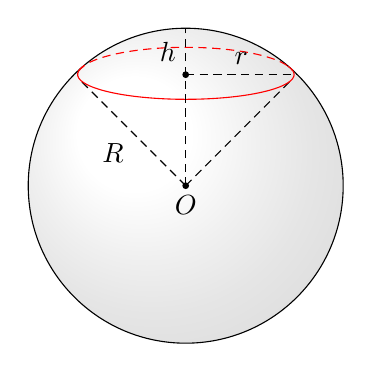
\begin{tikzpicture}[]
  \coordinate (O) at (0,0);
\coordinate (1) at (0,1.41);
\coordinate (2) at (0,2);
\coordinate (3) at (1.41,1.41);
  % ball background color
  \shade[ball color = white, opacity = 0.2] (0,0) circle [radius = 2cm];
  % ball
  \draw (O) circle [radius=2cm];
  % label of ball center point
  \filldraw (O) circle (1pt) node[below] {$O$};
  % radius
  \draw[densely dashed] (O) to [edge label = $R$] (-1.33,1.33);
  \draw[densely dashed] (O) -- (1.33,1.33);
  % cut of ball surface
  %\draw[red] (-1.35,1.47) arc [start angle = 140, end angle = 40, x radius = 17.6mm, y radius = 14.75mm];	% top
  \draw[red, densely dashed] (-1.36,1.46) arc [start angle = 170, end angle = 10, x radius = 13.8mm, y radius = 3.6mm];
  \draw[red] (-1.29,1.52) arc [start angle=-200, end angle = 20, x radius = 13.75mm, y radius = 3.15mm];
\filldraw (1) circle (1pt);
\draw (0.0,1.7) node[left] {$h$};
\draw[densely dashed] (1) to [edge label = $r$] (3);
\draw[densely dashed] (O) -- (2);
  % label of cut of ball surface
  %\draw (-1.2,2.2) -- (-0.53,1.83) node at (-1.37,2.37) {$A$};
\end{tikzpicture}
\end{minipage}
\begin{minipage}[t]{0.49\linewidth}
\centering
\begin{tikzpicture}[]
  \coordinate (O) at (0,0);
\coordinate (1) at (0,1.41);
\coordinate (2) at (0,2);
\coordinate (3) at (1.41,1.41);
  \draw (O) circle [radius=2cm];
  % label of ball center point
  \filldraw (O) circle (1pt);
  \draw[densely dashed] (O) to (3);
  \filldraw (1) circle (1pt);
\draw (0.0,0.7) node[left] {$u$};
\draw[densely dashed] (1) to [edge label = $r$] (3);
\draw[densely dashed] (O) -- (2);
\draw (0,2) coordinate (a) (0,0) coordinate (b) (1.41,1.41) coordinate (c) pic["$\theta$", draw,<-, angle eccentricity=1.5, angle radius=0.5cm]{angle=c--b--a};
\end{tikzpicture}
\end{minipage}
\end{figure} 

先求球冠的面积公式, 假设球半径为 $ R $, 球冠高度为 $ h $, 则取球冠上的一圈, 半径为 $ r = R\sin\theta $, 一圈长度为 $ 2\pi r = 2\pi R\sin\theta$, 宽度为 $ R \text{d}\theta $, 面积微元是 $ 2\pi R^2\sin\theta\text{d}\theta $. 
令 $ u = R\cos\theta $, 则 $ \text{d}u = -R\sin\theta\text{d}\theta $. 当 $ \theta $ 从 0 增加时, $ u $ 的变化范围是 $ R $ 到 $ R-h $. 面积为
\[ \int_{0}^\Theta {2\pi R^2\sin\theta\text{d}\theta} = \int_{R}^{R-h}{-2\pi R\text{d}u} = 2\pi Rh .\]

将这些向量起点挪到原点, 每个向量对应一个张角 $ 45 \degree $ (单侧张角 $ 22.5 \degree $) 的圆锥. 每个圆锥在单位球上截出一个球冠, 如果有两个球冠相交, 说明对应的两个向量夹角小于 $ 45 \degree $.

二倍角公式: $ \cos 2x = 2 \cos^2 x - 1 $, 得半角公式 $ \cos x = \sqrt{ \dfrac{\cos 2x+1}{2} } $

球冠高度为 \[ h = 1 - \cos 22.5\degree = 1 - \frac{\sqrt{2+\sqrt{2}}}{2} .\]

30 个球冠的面积为 \[ 30\times 2\pi Rh = 60\pi \left( 1 - \frac{\sqrt{2+\sqrt{2}}}{2} \right).\]

球的表面积为 $ 4\pi $. 比较发现 30 个球冠面积更大, 说明一定有球冠相交.

\newpage

%------------------------------------------------------------------------------%

\noindent 环球城市数学竞赛~ 1982 春季~ 初中组

集合 $ S $ 定义为: \[ S = \left\{ \frac{1}{k} \mid k = 1, 2, \cdots \right\} .\] 问是否存在由 $ S $ 中的不同元素构成的等差数列, 如果有, 可能有多少项.

~

解: 对于任意的正整数 $ n $, 可以构造数列 \[ \left\{ \frac{1}{n!}, \frac{2}{n!}, \cdots, \frac{n}{n!} \right\}. \]
则它是等差数列, 且都是 $ S $ 中的元素. 可见能构造任意长度的等差数列.

\newpage

%------------------------------------------------------------------------------%
\section{组合计数}

问题:圆周上有 $ n $ 个点,将它们两两相连得到一些弦,假设任意三条弦都不会相交于同一点,求这些弦之间一共有多少交点。

解:每个交点对应了两条弦,或者 4 个顶点,考虑圆周上任意 4 个点,它们之间可以有且只有一种情况能产生两条弦在圆内相交的情况。也就是说,一个 4 个点的组合与圆内弦的交点是一一对应的,所以交点共有 $ C_n^4 $ 个。

\vbox{}

问题:圆周上有 $ n $ 个点,将它们两两相连得到一些弦,假设任意三条弦都不会相交于同一点,求这些弦把圆分成多少个区域。

解:初始时有一个区域,每增加一条弦,会多出一个区域,现在考虑弦之间的交点。假如圆内已经有了一些弦,再画一条弦,可能会与其中的一些产生交点。画的过程中,从新弦的一个端点出发,如果没有产生新的交点,那么同样只会多出一个区域,而每产生一个交点,会额外分出一个区域。所以区域的总数为 $ 1 + C_n^2 + C_n^4 $,后面两项分别是弦的个数和交点的个数。

注: 当$n=1,2,3,4,5$时, 结果分别是$1, 2, 4, 8, 16$, 但当$n=6$时, 结果是$31$.


\newpage

%------------------------------------------------------------------------------%

问题:$ n $ 是给定的正整数,求有多少种正整数的组合 $ (i,j,k,h) $,满足:
\[ 1\le i < j \le k < h \le n+1 .\]

解:直接解法考虑 $ j=k $ 和 $ j\neq k $ 两种情况,分别相当于从 $ n+1  $ 个数中选 3 个和 4 个数,方法数为 $ C_{n+1}^3 + C_{n+1}^4 = C_{n+2}^4 $.

另一种思路:问题等价于求有多少个正整数的组合 $ (i,j,k',h') $ 满足:
\[ 1\le i < j < k' < h' \le n+2 .\]
直接得到答案。


\vbox{}

问题:罐子中有 $ n $ 个黑球和 $ n $ 个白球,每次从罐子里拿出一个球,直到取完,取球过程中,至少出现一次取出的白球多于取出的黑球的取法有多少种。

解:考虑罐子里有 $ n + 1 $ 个白球和 $ n - 1 $ 个黑球的取球序列,总会出现取出的白球个数多于黑球的情况,第一次出现时,取出的球中白球比黑球多 1 个,剩下的球中也是白球比黑球多 1 个。现在将剩下的球黑白颠倒,对应了原问题的所求情况。所以取法共有 $ C_{2n}^{n-1} $ 种。

\vbox{}

问题:由数字 0 和 1 组成的序列中,如果相邻两位的数不一样称为一次翻转,一个长度为 $ m $ 的序列恰好有 $ n $ 次翻转的情况有多少种。

解:直接法,长度为 $ m $ 的序列有 $ m - 1 $ 个间隙,每个间隙都可以翻转,确定了 $ n $ 次翻转的位置,第一位是 0 或 1 分别对应了一个序列,所以情况有 $ 2 C_{m-1}^n $ 种。

\vbox{}

问题:由数字 0 和 1 组成的长度为 $ m $ 的序列中,一个 0 紧跟在一个 1 后面的这样一个二元组出现了 $ n $ 次,求有多少种情况。

解:出现一个 01 后,下次再要遇到一个 01 之前,需要经历一次从 1 到 0 的翻转。因为 01 出现了 $ n $ 次,序列第一位和最后一位的数字与 1 到 0 的翻转出现的次数如下:

第一位是 0,最后一位也是 0,10 出现 $ n $ 次;

第一位是 0,最后一位是 1,10 出现 $ n - 1 $ 次;

第一位是 1,最后一位是 0,10 出现 $ n + 1 $ 次;

第一位是 1,最后一位也是 1,10 出现 $ n $ 次;

\noindent 所有情况加起来是 $ C_{m-1}^{2n} + C_{m-1}^{2n-1} + C_{m-1}^{2n+1} + C_{m-1}^{2n} = C_m^{2n} + C_m^{2n+1} = C_{m+1}^{2n+1} $.

另一个思路是考虑在原来序列前面补一个 1,后面补一个 0,这样原序列出现 $ n $ 次 01 等价于新序列发生 $ 2n+1 $ 次翻转(其中 0 到 1 发生 $ n $ 次,1 到 0 发生 $ n + 1 $ 次),而间隙有 $ m + 1 $ 个,所以可能的情况有 $ C_{m+1}^{2n+1} $ 种。

\vbox{}

问题:$ m $ 个白球和 $ n $ 个黑球排成一列,黑球不相邻的情况有多少种。

解:白球之间加上两端共有 $ m + 1$ 个空隙,选 $ n $ 个插入黑球,方法数为 $ C_{m+1}^n $.

另一个思路:除最后一个黑球外,其他黑球都吃掉它后面的一个白球,这样一共还剩 $ m + 1 $ 个球,将它们任意排列,之后除最后一个黑球之外的黑球再吐出一个白球,这就对应了一种黑球不相邻的序列。

\vbox{}

问题:圆周上有 $ m $ 个白球,编号为 $ 1,2,\cdots,m $,选出 $ n $ 个染黑,要求黑球不相邻,求方法数。

解:从 1 号断开,分两种情况。

(1) 1 号是白球,剩下的球中有 $ m - 1 - n $ 个白球和 $ n $ 个黑球,根据上一题结论,方法数为 $ C_{m-n}^n $;

(2) 1 号是黑球,从而 2 号和 $ m $ 号是白球,剩下的球中有 $ m - n - 2 $ 个白球和 $ n - 1 $ 个黑球,方法数为 $ C_{m-n-1}^{n-1} $.

加起来即可:
\begin{align*}
C_{m-n}^n + C_{m-n-1}^{n-1} &= 2C_{m-n}^n - C_{m-n-1}^n \\
& = \frac{2(m-n)!}{n!(m-2n)!} - \frac{(m-n-1)!}{n!(m-2n-1)!} \\
& = \frac{(m-n)!}{n!(m-2n)!}(2-\frac{m-2n}{m-n}) \\ 
& = \frac{m}{m-n} C_{m-n}^n
\end{align*}

\vbox{}

问题:三角形每条边被分成了 $ n $ 等分,连接这些分点,求图中有多少平行四边形。
\begin{figure*}[htbp]
\definecolor{sexdts}{rgb}{0.1803921568627451,0.49019607843137253,0.19607843137254902}
\definecolor{dtsfsf}{rgb}{0.8274509803921568,0.1843137254901961,0.1843137254901961}
\definecolor{rvwvcq}{rgb}{0.08235294117647059,0.396078431372549,0.7529411764705882}
\centering
\begin{minipage}[t]{0.49\linewidth}
\begin{tikzpicture}[line cap=round,line join=round,>=triangle 45,x=1cm,y=1cm,scale=0.8]
\clip(-4.5,-0.4) rectangle (4.95,5.15);
\draw [line width=1pt] (-4,0)-- (-2,4);
\draw [line width=1pt] (-2,4)-- (4,0);
\draw [line width=1pt] (4,0)-- (-4,0);
\draw [line width=1pt] (-2.25,3.5)-- (-1.25,3.5);
\draw [line width=1pt] (-2.5,3)-- (-0.5,3);
\draw [line width=1pt] (-2.75,2.5)-- (0.25,2.5);
\draw [line width=1pt] (1,2)-- (-3,2);
\draw [line width=1pt] (-3.25,1.5)-- (1.75,1.5);
\draw [line width=1pt] (2.5,1)-- (-3.5,1);
\draw [line width=1pt] (-3.75,0.5)-- (3.25,0.5);
\draw [line width=1pt] (-3,0)-- (-1.25,3.5);
\draw [line width=1pt] (-0.5,3)-- (-2,0);
\draw [line width=1pt] (-1,0)-- (0.25,2.5);
\draw [line width=1pt] (1,2)-- (0,0);
\draw [line width=1pt] (1,0)-- (1.75,1.5);
\draw [line width=1pt] (2.5,1)-- (2,0);
\draw [line width=1pt] (3,0)-- (3.25,0.5);
\draw [line width=1pt] (3,0)-- (-2.25,3.5);
\draw [line width=1pt] (-2.5,3)-- (2,0);
\draw [line width=1pt] (1,0)-- (-2.75,2.5);
\draw [line width=1pt] (-3,2)-- (0,0);
\draw [line width=1pt] (-1,0)-- (-3.25,1.5);
\draw [line width=1pt] (-3.5,1)-- (-2,0);
\draw [line width=1pt] (-3,0)-- (-3.75,0.5);
\begin{scriptsize}
\draw [fill=rvwvcq] (-4,0) circle (1.5pt);
\draw[color=rvwvcq] (-4.2,-0.2) node {$A$};
\draw [fill=rvwvcq] (4,0) circle (1.5pt);
\draw[color=rvwvcq] (4.2,-0.2) node {$B$};
\draw [fill=rvwvcq] (-2,4) circle (1.5pt);
\draw[color=rvwvcq] (-1.9171333333333305,4.229688888888887) node {$C$};
\end{scriptsize}
\end{tikzpicture}
\end{minipage}
\begin{minipage}[t]{0.49\linewidth}
\begin{tikzpicture}[line cap=round,line join=round,>=triangle 45,x=1cm,y=1cm,scale=0.8]
\clip(-4.5,-0.4) rectangle (4.95,5.15);
\draw [line width=1pt] (-4,0)-- (-2,4);
\draw [line width=1pt] (-2,4)-- (4,0);
\draw [line width=1pt] (4,0)-- (-4,0);
\draw [line width=1pt] (-2.25,3.5)-- (-1.25,3.5);
\draw [line width=1pt] (-2.5,3)-- (-0.5,3);
\draw [line width=1pt] (-2.75,2.5)-- (0.25,2.5);
\draw [line width=1pt] (1,2)-- (-3,2);
\draw [line width=1pt] (-3.25,1.5)-- (1.75,1.5);
\draw [line width=1pt] (2.5,1)-- (-3.5,1);
\draw [line width=1pt] (-3.75,0.5)-- (3.25,0.5);
\draw [line width=1pt,color=dtsfsf] (-3,0)-- (-1.25,3.5);
\draw [line width=1pt,color=dtsfsf] (-0.5,3)-- (-2,0);
\draw [line width=1pt] (-1,0)-- (0.25,2.5);
\draw [line width=1pt] (1,2)-- (0,0);
\draw [line width=1pt] (1,0)-- (1.75,1.5);
\draw [line width=1pt] (2.5,1)-- (2,0);
\draw [line width=1pt] (3,0)-- (3.25,0.5);
\draw [line width=1pt,color=sexdts] (3,0)-- (-2.25,3.5);
\draw [line width=1pt] (-2.5,3)-- (2,0);
\draw [line width=1pt,color=sexdts] (1,0)-- (-2.75,2.5);
\draw [line width=1pt] (-3,2)-- (0,0);
\draw [line width=1pt] (-1,0)-- (-3.25,1.5);
\draw [line width=1pt] (-3.5,1)-- (-2,0);
\draw [line width=1pt] (-3,0)-- (-3.75,0.5);

\begin{scriptsize}
\draw (-3.0,-0.25) node {$i$};
\draw (-2.0,-0.25) node {$j$};
\draw (1.0,-0.25) node {$k$};
\draw (3.0,-0.25) node {$h$};

\draw [fill=rvwvcq] (-4,0) circle (1.5pt);
\draw[color=rvwvcq] (-4.2,-0.2) node {$A$};
\draw [fill=rvwvcq] (4,0) circle (1.5pt);
\draw[color=rvwvcq] (4.2,-0.2) node {$B$};
\draw [fill=rvwvcq] (-2,4) circle (1.5pt);
\draw[color=rvwvcq] (-1.9171333333333305,4.229688888888887) node {$C$};
\end{scriptsize}
\end{tikzpicture}
\end{minipage}
\end{figure*}

解:这些平行四边形有 3 类,每一类的两组对边分别与原三角形的两条边平行,先考虑其中一类平行四边形,它的边分别与 $ AC $ 和 $ BC $ 平行。

延长与 $ AC $ 平行的边,与 $ AB $ 交于 $ i,j $ 两个分点,再延长与 $ BC $ 平行的边,与 $ AB $ 交于 $ k,h $ 两个分点。设 $ A,B $ 两点分别是线段 $ AB $ 的第 1 和第 $ n + 1 $ 个分点,则构成平行四边形的充要条件是 $ 1 \le i < j \le k < h \le n+1 $.

所以总个数为 $ 3C_{n+2}^4 $.

\vbox{}

问题: $m$ 个球放进 $n$ 个不同的罐子, 每个罐子至少有一个球, 有多少种可能性?

解: $m$ 个球排成一列, 相邻两球中间有一个空隙, 相当于要在这 $m-1$ 个空隙种选出 $n-1$ 个放入隔板, 隔板将一列球分成了 $n$ 段, 每个罐子里放入对应的段. 总共有 $C_{m-1}^{n-1}$ 种情况.


\vbox{}

问题: $m$ 个球放进 $n$ 个不同的罐子, 可以有空罐子, 有多少种可能性?

解: 再加入 $n$ 个球, 变成共 $m+n$ 个球放入 $n$ 个罐子, 每个罐子至少一个球的问题. 情况数是 $C_{m+n-1}^{n-1}$.

\newpage

%------------------------------------------------------------------------------%

可重复计数的证明:

从 $ [1,m] $ 范围取 $ n $ 个数,取出的数可以重复,总的取法有 $ C_{m+n-1}^n $ 种。 

例如:投 5 个骰子,一共会出现 $ C_{10}^{5} $ 种情况。

\begin{proof}

将取出来的数从小到大排列,设为 $ 1 \le a_1 \le a_2 \le \cdots \le a_n \le m $,等价于从 $ [1,m-n+1] $ 范围取 $ n $ 个数,满足 $ a_1 < a_2 < \cdots < a_n $,所以取法有 $ C_{m+n-1}^n $ 种。

\end{proof}

另一种思路:考虑 $ m - 1 $ 个白球和 $ n $ 个黑球排成一列,将第 $ i $ 个黑球之前的白球数量加 1 视为原问题中取出的第 $ i $ 大的数,答案就是 $ C_{m+n-1}^n $.

注意到第二种思路可以用来计算整数拆分的方法数。

\newpage

%------------------------------------------------------------------------------%

有一个宝箱,上面锁了一些锁,这些锁的钥匙被 $ n $ 个人保管,每个人有相同数量的钥匙,每个钥匙能开其中的一把锁。任意 $ k $ 个人将钥匙凑在一起可以打开全部的锁,而任意 $ k - 1 $ 个人的钥匙都不能打开全部锁。求至少需要多少把锁,以及此时每个人有多少把钥匙,以及此时任选 $ i $ 个人的组合中每个人都有的钥匙有多少种。

思路:考虑一个特定的人 $ A $,剩下 $ n - 1 $ 个人中任选 $ k - 1 $ 个人都会缺钥匙,而 $ A $ 正好有他们缺的钥匙。

注意到任意两个 $ k - 1 $ 人组合都不会缺同一把钥匙,如若不然,则这两个组合的并集至少有 $ k $ 个人,但他们还是缺一把钥匙,矛盾。

这就说明了 $ A $ 至少拥有剩下 $ n - 1 $ 个人中任选 $ k - 1 $ 个人的组合个数那么多把钥匙,也就是 $ C_{n-1}^{k-1} $。其他人的情况也一样,这样每个人都至少有这么多把钥匙。

另一方面,对于特定的一把锁,任意选 $ k $ 个人都能找到开它的钥匙,这就说明这个锁有 $ n - k + 1 $ 把钥匙。

综上所述,钥匙种类数量为 
\begin{align*} 
\frac{n}{n-k+1}C_{n-1}^{k-1} &= \frac{n}{n-k+1}\frac{(n-1)!}{(k-1)!(n-k)!} \\
				&=\frac{n!}{(k-1)!(n-k+1)!} \\
				&=C_n^{k-1}
\end{align*}

再考虑 $ n $ 个人取 $ k - 1 $ 个人的组合,这些组合都至少缺一个锁的钥匙,且没有两个组合会缺同一个锁的钥匙,所以锁至少有 $ C_n^{k-1} $ 个。













